% Exercises: tikz libraries (positioning, arrows.meta, shapes, calc, fit, matrix), nodes, paths, foreach, scopes.
\documentclass{article}
\usepackage{tikz}\usetikzlibrary{positioning,arrows.meta,shapes.geometric,calc,fit,matrix,decorations.pathmorphing}
\begin{document}
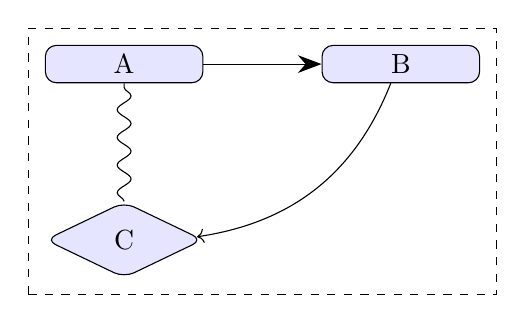
\begin{tikzpicture}[node distance=1.5cm,box/.style={draw,rounded corners,minimum width=2cm,fill=blue!10}]
\node[box](a){A};\node[box,right=of a](b){B};\node[box,below=of a,diamond](c){C};
\draw[-{Stealth[length=3mm]}](a)--(b);\draw[->,bend left](b)to(c);\draw[decorate,decoration=snake](c)--(a);
\node[draw,dashed,fit=(a)(b)(c),inner sep=6pt]{};
\end{tikzpicture}
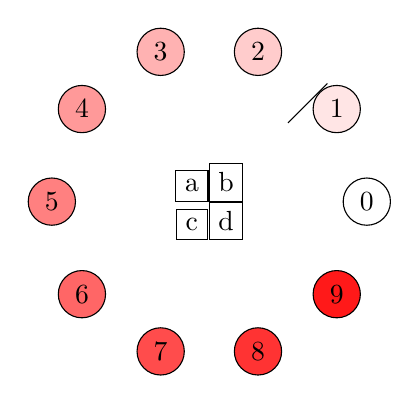
\begin{tikzpicture}\foreach\i in {0,...,9}{\draw[fill=red!\the\numexpr\i*10\relax](\i*36:2)circle(.3)node{\i};}
\coordinate(p)at(0,0);\draw($(p)+(1,1)$)--($(p)!.5!(3,3)$);
\matrix[matrix of nodes,nodes={draw}]{a&b\\c&d\\};\end{tikzpicture}
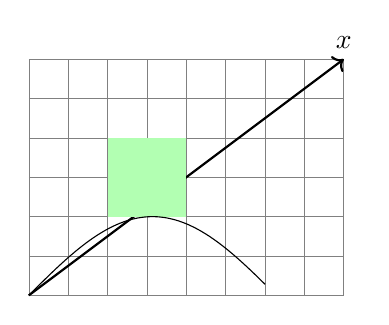
\begin{tikzpicture}\draw[step=.5,gray,very thin](0,0)grid(4,3);\draw[thick,->](0,0)--(4,3)node[above]{$x$};
\path[fill=green!30](1,1)rectangle(2,2);\draw plot[smooth,domain=0:3]({\x},{sin(\x r)});\end{tikzpicture}
\end{document}
